\documentclass[tikz,border=6pt]{standalone}
\usepackage[T1]{fontenc}
\usepackage{lmodern}
\usepackage{amsmath}
\usetikzlibrary{positioning,arrows.meta,fit,calc}
% Design of koblitz-n83-rankcut-20261016 (frozen protocol.json). Not a result.
\begin{document}
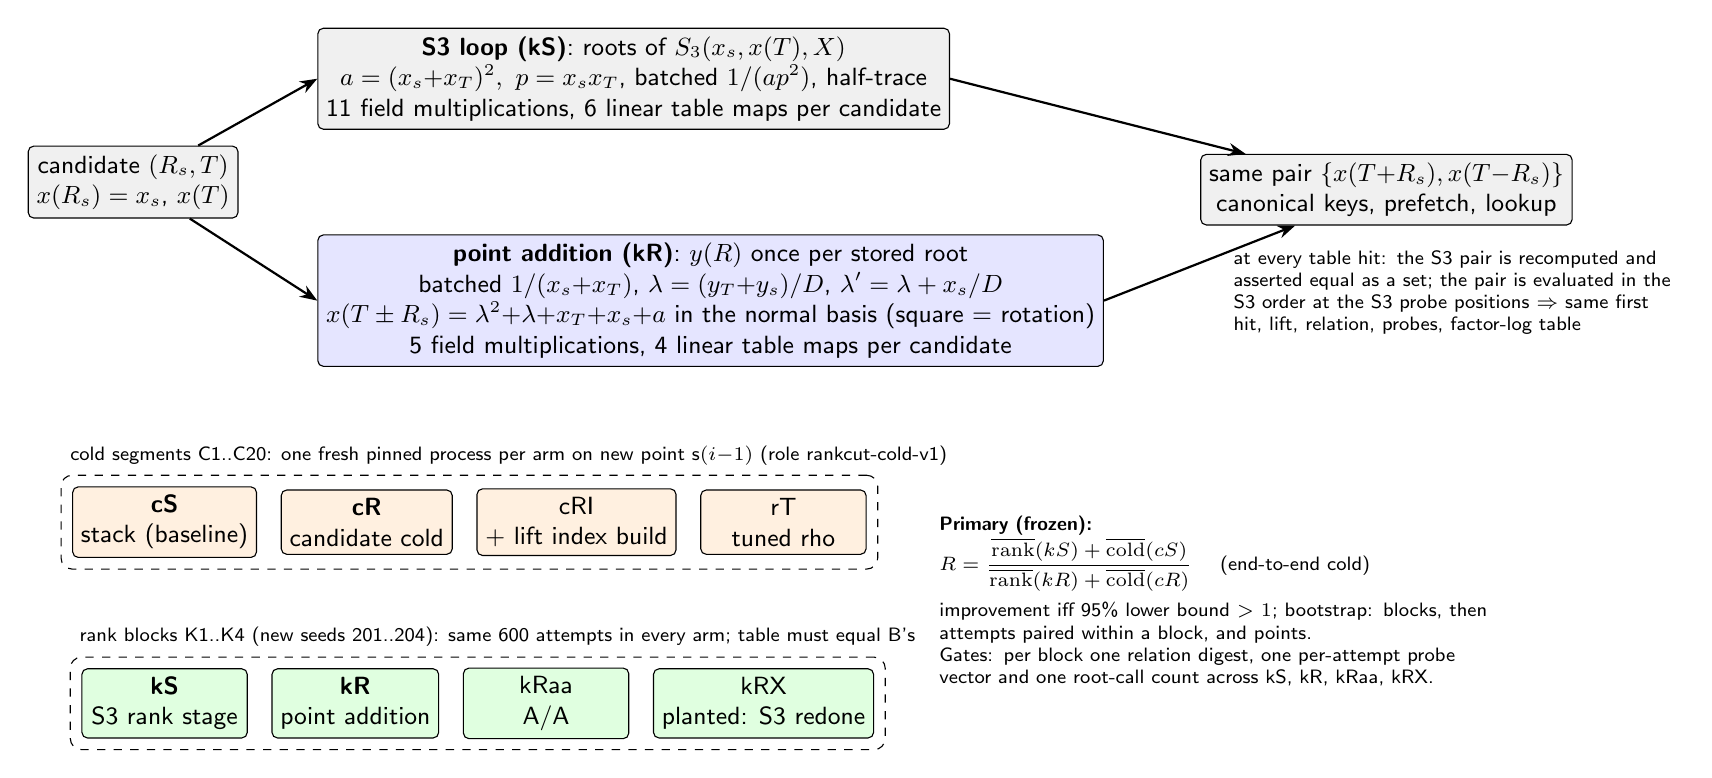
\begin{tikzpicture}[
  font=\sffamily\small,
  box/.style={draw, rounded corners=2pt, align=center, minimum height=8mm, inner sep=3pt},
  base/.style={box, fill=gray!12},
  add/.style={box, fill=blue!10},
  arm/.style={box, fill=orange!12, minimum width=21mm},
  rank/.style={box, fill=green!12, minimum width=21mm},
  arr/.style={-{Stealth[length=2.2mm]}, thick},
  note/.style={align=left, font=\sffamily\scriptsize}
]
% One candidate of one state: stored root R_s (Frobenius shift s), rank target T
\node[base] (in) {candidate $(R_s, T)$\\$x(R_s)=x_s$, $x(T)$};
\node[base, above right=2mm and 10mm of in] (s3) {\textbf{S3 loop (kS)}: roots of $S_3(x_s, x(T), X)$\\
$a=(x_s{+}x_T)^2,\ p=x_s x_T$, batched $1/(a p^2)$, half-trace\\11 field multiplications, 6 linear table maps per candidate};
\node[add, below right=2mm and 10mm of in] (pa) {\textbf{point addition (kR)}: $y(R)$ once per stored root\\
batched $1/(x_s{+}x_T)$, $\lambda=(y_T{+}y_s)/D$, $\lambda'=\lambda+x_s/D$\\$x(T\pm R_s)=\lambda^2{+}\lambda{+}x_T{+}x_s{+}a$ in the normal basis (square = rotation)\\5 field multiplications, 4 linear table maps per candidate};
\draw[arr] (in) -- (s3.west); \draw[arr] (in) -- (pa.west);
\node[base, anchor=west] (keys) at ($(pa.east)!0.5!(s3.east) + (22mm,0)$) {same pair $\{x(T{+}R_s), x(T{-}R_s)\}$\\canonical keys, prefetch, lookup};
\draw[arr] (s3.east) -- (keys); \draw[arr] (pa.east) -- (keys);
\node[note, anchor=north west, text width=56mm] (ex) at ($(keys.south west)+(3mm,-2mm)$) {at every table hit: the S3 pair is recomputed and asserted equal as a set;
the pair is evaluated in the S3 order at the S3 probe positions $\Rightarrow$ same first hit, lift, relation, probes, factor-log table};

% Cold arms
\node[arm, below=34mm of in, xshift=4mm] (cS) {\textbf{cS}\\stack (baseline)};
\node[arm, right=3mm of cS] (cR) {\textbf{cR}\\candidate cold};
\node[arm, right=3mm of cR] (cRI) {cRI\\+ lift index build};
\node[arm, right=3mm of cRI] (rT) {rT\\tuned rho};
\node[draw, dashed, rounded corners, fit=(cS) (rT), inner sep=4pt, label={[note, anchor=south west]north west:{cold segments C1..C20: one fresh pinned process per arm on new point s$(i{-}1)$ (role rankcut-cold-v1)}}] (cold) {};

% Rank arms
\node[rank, below=14mm of cS] (kS) {\textbf{kS}\\S3 rank stage};
\node[rank, right=3mm of kS] (kR) {\textbf{kR}\\point addition};
\node[rank, right=3mm of kR] (kRaa) {kRaa\\A/A};
\node[rank, right=3mm of kRaa] (kRX) {kRX\\planted: S3 redone};
\node[draw, dashed, rounded corners, fit=(kS) (kRX), inner sep=4pt, label={[note, anchor=south west]north west:{rank blocks K1..K4 (new seeds 201..204): same 600 attempts in every arm; table must equal B's}}] (rk) {};

\node[note, right=8mm of rT, text width=70mm, yshift=-10mm] (eq) {\textbf{Primary (frozen):}\\
$R = \dfrac{\overline{\mathrm{rank}}(kS) + \overline{\mathrm{cold}}(cS)}{\overline{\mathrm{rank}}(kR) + \overline{\mathrm{cold}}(cR)}$ \quad (end-to-end cold)\\[1mm]
improvement iff 95\% lower bound $>1$; bootstrap: blocks, then attempts paired within a block, and points.\\
Gates: per block one relation digest, one per-attempt probe vector and one root-call count across kS, kR, kRaa, kRX.};
\end{tikzpicture}
\end{document}
